\section{Method}

Our method works on top of existing $EM$ agglomeration algorithms such as \textit{NeuroProof} or \textit{GALA} (CITE BOTH). First we use a 3D U-net to generate voxel affinities predicting the probability that two voxels belong to the same neuron. The \textit{zwatershed} algorithms takes these affinities and generates an oversegmentation of the neurons (CITE). \textit{NeuroProof} agglomerates these supervoxels by training a multi-level random forest classifier. We use a low threshold for neuroproof to generate an oversegmentation. 

NEED TO ADD BETTER OVERVIEW

\subsection{Preprocessing}

Our pipeline builds a level on top of current agglomeration techniques. Our goal is to identify and merge segments based on their overall shape. Figure (ADD FIGURE) shows two examples of nearby segments output by \textit{NeuroProof}. The right pair should merge and the left pair should not.  

We consider the skeletons of the segments. We use the teasFigure (ADD FIGURE) shows two examples of skeletons generated for two neuron segments. The skeletons are generated using the TEASER: Tree-structure Extraction Algorithm for Accurate and Robust Skeletons (CITE TEASER). The algorithm iteratively chooses locations that are the furthest distance $d$ from the boundary of the segment. Each locations becomes a ``joint" and a sphere of radius $d$ centered at the joint is masked out. The algorithm continually finds points and removes the corresponding sphere until every point with a distance greater than $d^*$ is removed. We use a $d^*$ of 50 voxels which was the standard parameter from the original paper (Is it?). 

We use the above skeletons to extract feature locations to consider merges. The algorithm is described in the pseudocode in (ADD CITE).

ADD IN PSEUDOCODE

\begin{itemize}
	
	
	
	\item Skeletonization
	\item Feature generation
\end{itemize}

\subsection{Error Detection}

\begin{figure*}[t]
	\centering
	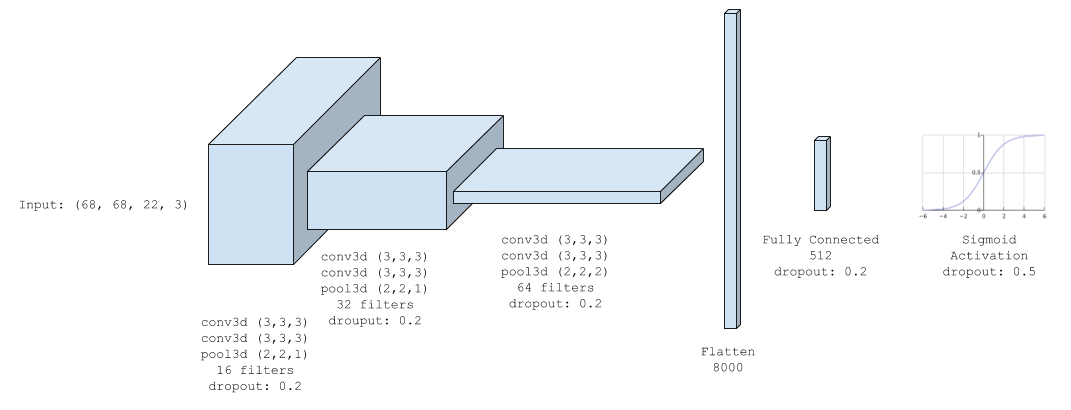
\includegraphics[width=0.8\linewidth]{figures/architecture.png}
	\caption{The architecture for the neural networks follows the \textit{VGG} style of double convolutions followed by a max pooling operation. The number of filters doubles each layer leading to a fully connected layer and a sigmoid activation function.}
	\label{fig:architecture}
\end{figure*}

NEED TO CITE VGG, LeakyReLU, BatchNormalization

The above skeletonization strategies produces locations in 3D that require further consideration. From these locations we extract a region of $800nm \times 800nm \times 800nm$ and resample the segmentations to fit in a box of $18 \times 52 \times 52$ voxels. Consider a location corresponding to a potential merge between labels $l_1$ and $l_2$. The input to the neural network is a three binary channel cube of size $3 \times 18 \times 52 \times 52$. The first channel is $1$ if the voxel belongs to $l_1$. The second channel is 1 if the voxel belongs to $l_2$. The third channel is $1$ if the voxel belongs to either $l_1$ or $l_2$. 

We train a 3D convolutional neural network on the the generated examples. The network has four layers of double convolutions followed by a max pooling step. The filter sizes are $(3, 3, 3)$ and the max pooling is by a factor of $2$ for every level in the $x$ and $y$ dimensions. We downsample the $z$ dimension only in the final two layers. The number of channels is $16$ for the first layer and each subsequent layer has twice as many channels. The output of the convolutions is flattened and input into two dense layers. We apply batch normalization after every convolution, pooling, and dense layer except for the final layer. We use the \textit{LeakyReLU} activation function with $\alpha = 0.001$. We use the \textit{Adam} optimizer with an initial learning rate of $0.001$, $\beta_1 = 0.99$, $\beta_2 = 0.999$, and a weight decay of $5*10^{-8}$. The loss function is binary crossentropy. We use a batch size of 20.  

Since the datasets have a limited number of examples, we augment the examples by considering all combinations with rotations along the $xy$-plane and mirrors along the $yz$- and $xy$- planes. This produces 16 times more training data.

\begin{itemize}
	\item CNN Architecture
	\item Classifier Inputs
\end{itemize}

\subsection{Agglomeration}

The above neural network produces probabilities that two nearby segments belong to the same neuron. To use the graph-based optimization algorithms we need to take the oversegmentation and construct a graph. We generate one node for every segment. The skeletonization algorithm generates edges between nodes. 

\begin{itemize}
	\item Error Correction
\end{itemize}
